\documentclass{letter}
\usepackage{wallpaper}
\usepackage{geometry}
\usepackage{xcolor}
\usepackage{tikz}
\usepackage[T1]{fontenc}
\usepackage[scaled]{helvet}
\usepackage{fontawesome5}
\usepackage{hyperref}
\usepackage[none]{hyphenat}

\renewcommand{\familydefault}{\sfdefault}

\geometry{
  paperwidth=\dimexpr\textwidth+\marginparsep+\marginparwidth\relax,
  paperheight=\dimexpr\textheight+\footskip\relax,
  left=20pt,
  right=20pt,
  top=0pt,
  bottom=0pt,
  nohead,
  nofoot,
  nomarginpar
}

\ThisCenterWallPaper{1.5}{data/cvbg.png}

\begin{document}

\begin{minipage}[t]{0.40\textwidth}
\setlength{\baselineskip}{1.5\baselineskip}
\color{white}

\hspace{0.7cm}
\begin{tikzpicture}
    \draw[line width=2pt] (0.05, 1) circle (2cm);
    \clip (0.05,1) circle (2cm);
    \node[inner sep=0pt, scale=1.5] (image)
        {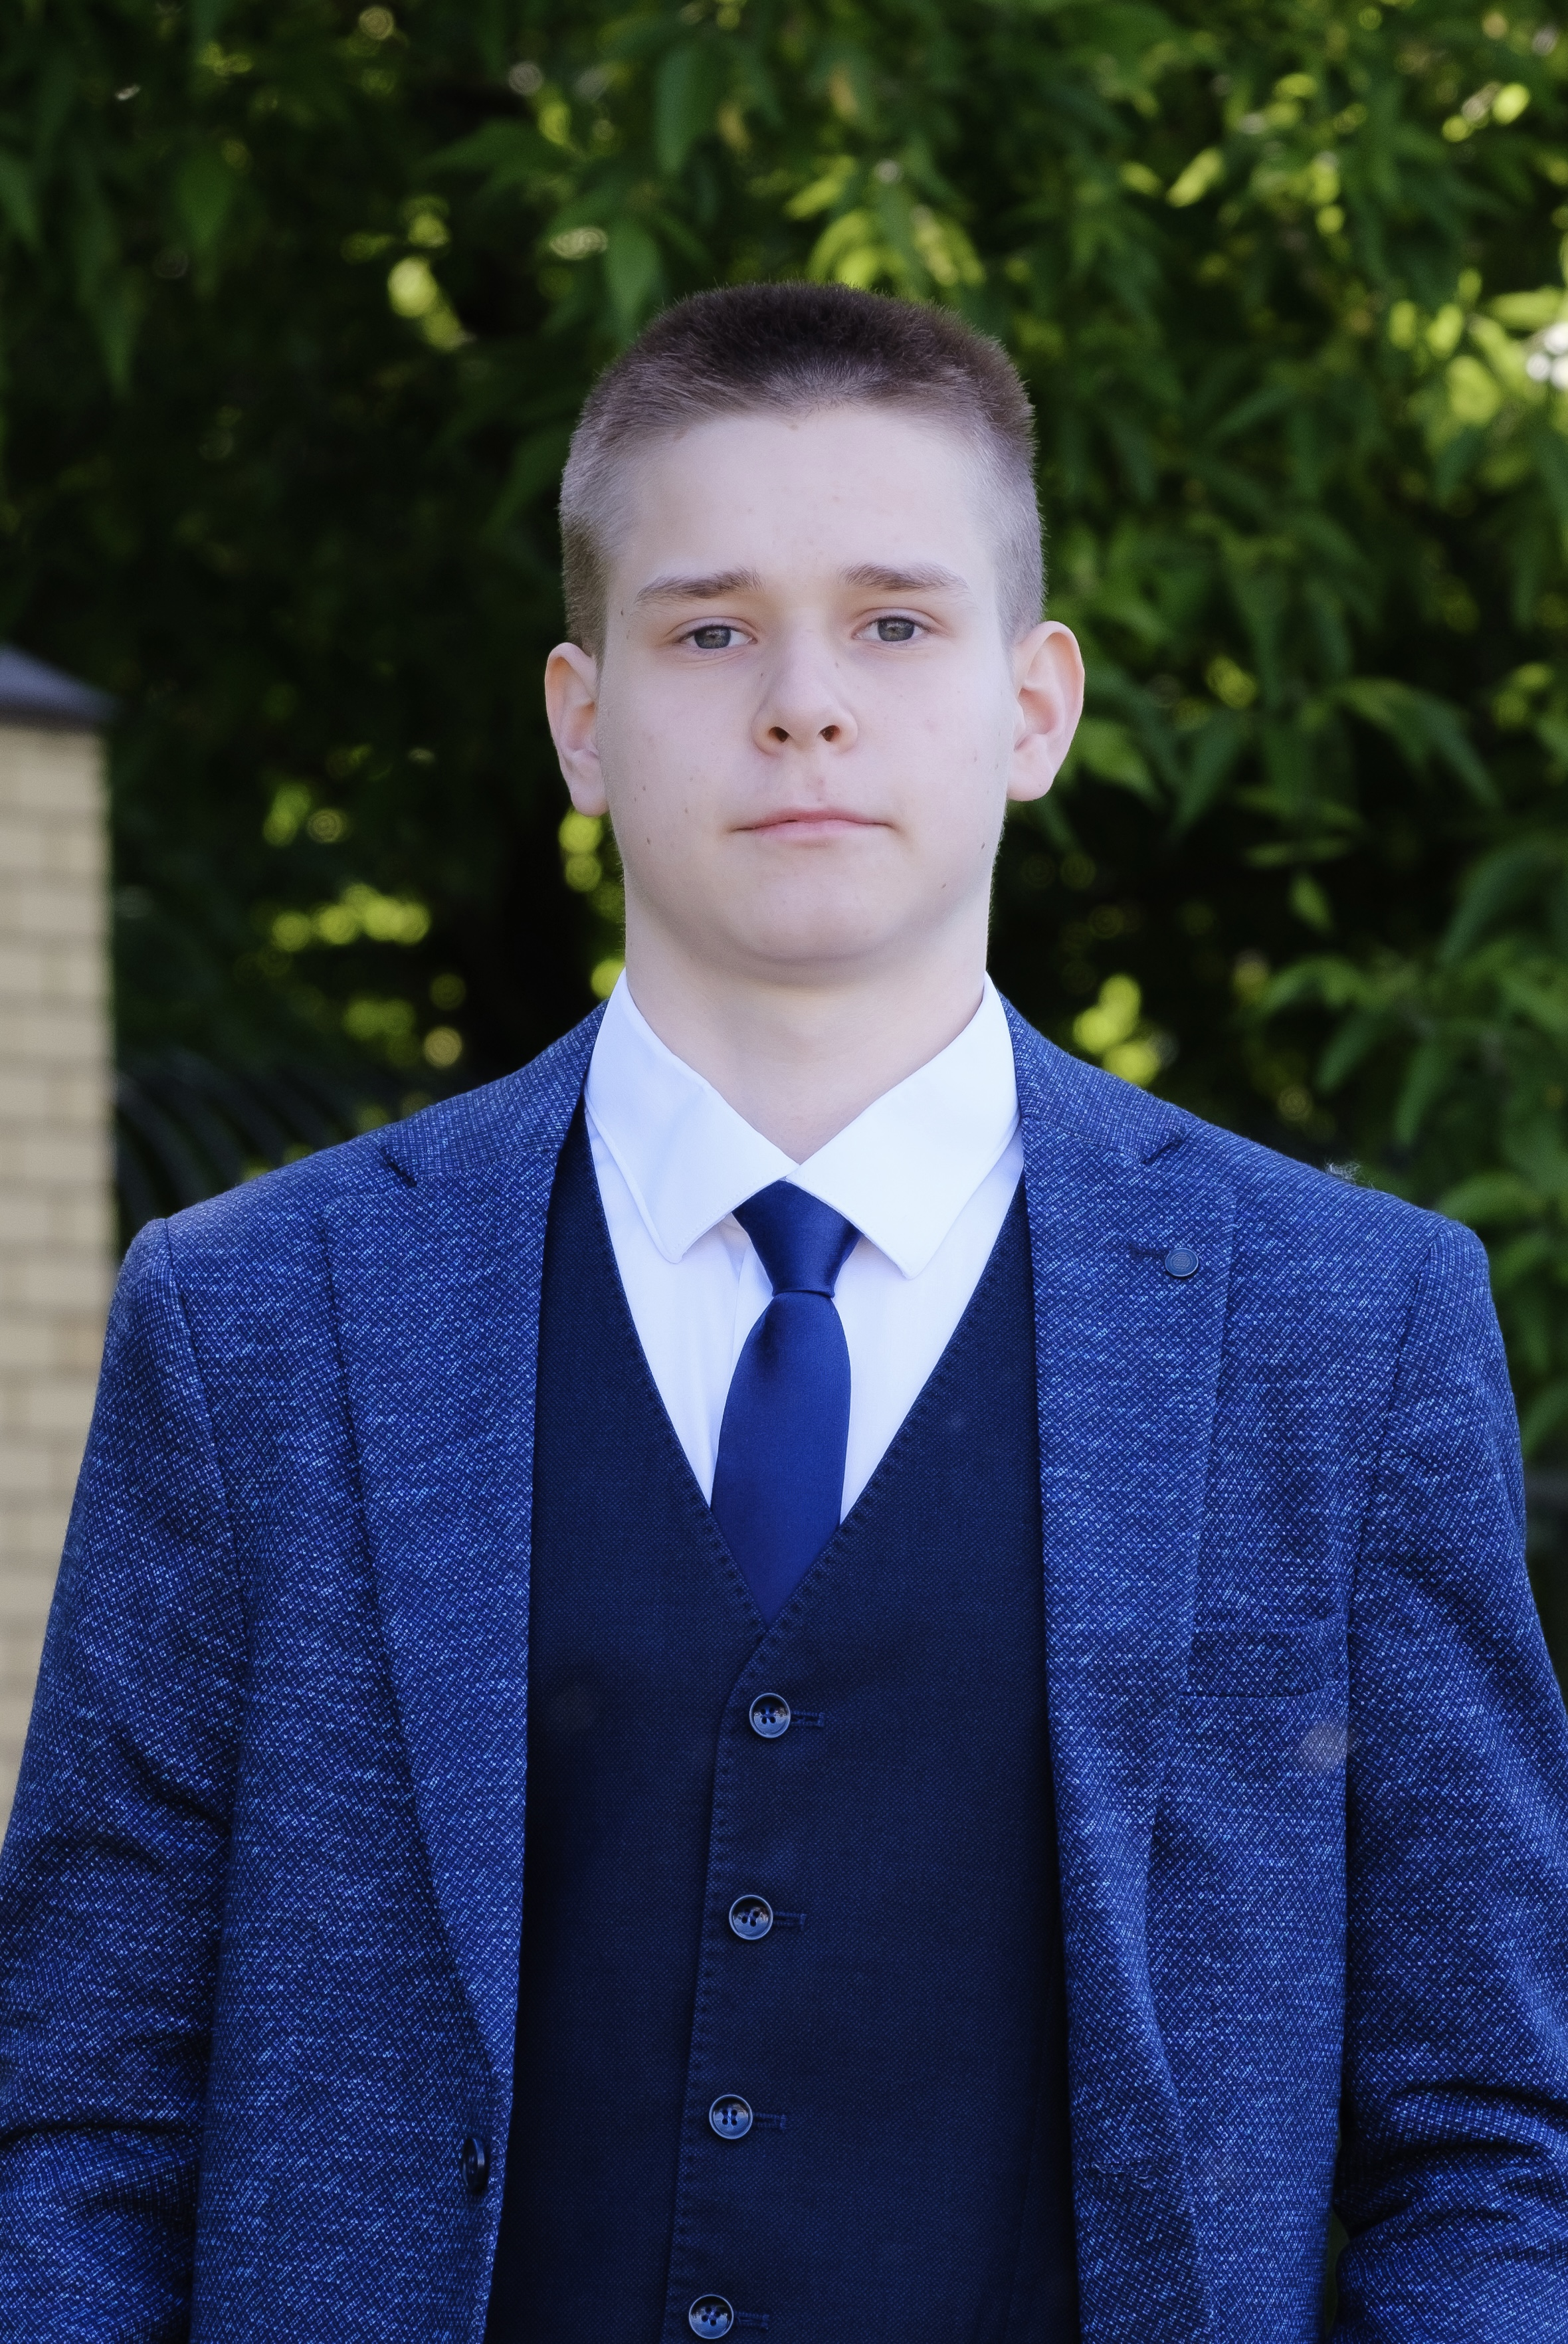
\includegraphics[width=3cm]{data/self.jpeg}};
\end{tikzpicture}

\rule{\linewidth}{0.4pt}

\faPhone \quad +7-910-350-06-98

\faEnvelope \quad \href{mailto:tolik_rogov@bk.ru}{tolik\_rogov@bk.ru}

\faMapMarker \quad Moscow

\rule{\linewidth}{0.4pt}

{\large Links}

\faGithub \quad \href{https://github.com/TolikRogov}{TolikRogov}

\rule{\linewidth}{0.4pt}

{\large Skills}

\faCode \quad C

\faCode \quad Asm

\rule{\linewidth}{0.4pt}

{\large Tools}

\faCircleNotch  \quad git

\faCircleNotch  \quad Make/Cmake

\faCircleNotch  \quad Doxygen/Graphviz

\faCircleNotch  \quad radare2

\faCircleNotch  \quad \LaTeX

\rule{\linewidth}{0.4pt}

{\large Languages}

\faLanguage \quad Russian

\faLanguage \quad English B2

\end{minipage}
\hfill
\begin{minipage}[t]{0.60\textwidth}
\setlength{\baselineskip}{1.5\baselineskip}
\vspace{0.8cm}
{\huge Rogov Anatoliy}

{\large First year student of MIPT}

\vspace{0.5cm}

{\large Projects}
\rule{\linewidth}{0.4pt}

{\large \textbf{\href{https://github.com/TolikRogov/Language}{Language compiler}}}

{\small December 2024 - Tools: C, Cmake, HTML, Graphviz}

\begin{itemize}
    {\small
    \item Created language specification
    \item Lexical analysis with support for replacement table and detailed dump in debug mode
    \item Recursive descent parsing
    \item Support for tree standard
    \item Performing optimizations using middleware
    \item Representation in binary code for execution on the own \href{https://github.com/TolikRogov/Processor}{processor}
    }
\end{itemize}

{\large \textbf{\href{https://github.com/TolikRogov/Mandelbrot}{Mandelbrot}}}

{\small March 2025 - Tools: C/C++, Cmake, \LaTeX}

\begin{itemize}
    {\small
    \item Constructing a fractal of the mandelbrot set with the SFML library
    \item SIMD (AVX) computation optimizations
    \item Comparison of program execution time depending on the optimization level
    }
\end{itemize}

{\large Education}
\vspace{0.2cm}
\rule{\linewidth}{0.4pt}

{\textbf{Moscow Institute of Physics and Technology (MIPT)}}\\
\small Dolgoprudny, Russia, September 2024 - June 2028\\

\small First year student of the Faculty of Radio Engineering and Computer Technologies. \textbf{GPA}: 8.1/10.0\\

{\textbf{System programming and compiler technology course (MIPT)}}\\
\small Dolgoprudny, Russia, September 2024 - June 2025\\

\small Completed the first semester with \textbf{GPA}: 10.0/10.0\\

{\large Achievements}
\rule{\linewidth}{0.4pt}\\

\textbf{Prize-winner of the 2nd degree in Informatics at the Engineering Olympiad of Central Russia}\\
{\small Lipetsk, Russia, 2023}

\end{minipage}
\end{document}
